\chapter{Conclusion}

Après une mise à l'échelle des graphes afin d'éviter de laisser transparaître les différences de puissances de nos machines respectives, nous constatons que l'algorithme de recherche dichotomique (accompagné de l'algorithme de tri dichotomique) possède une tendance exponentielle, car il est de complexité $O(log(n^n + n'))$. Les autres algorithmes, eux, possédant une complexité $O(n)$ ont une tendance linéaire avec des pentes différentes, mais n’ont pas le même temps d'exécution (voir Figure \ref{fig:fig_conclusion}). On peut en conclure que même si des algorithmes distincts possèdent la même complexité ne signifie pas que le temps d'exécution sera le même.

\begin{figure}[H]
    \centering
        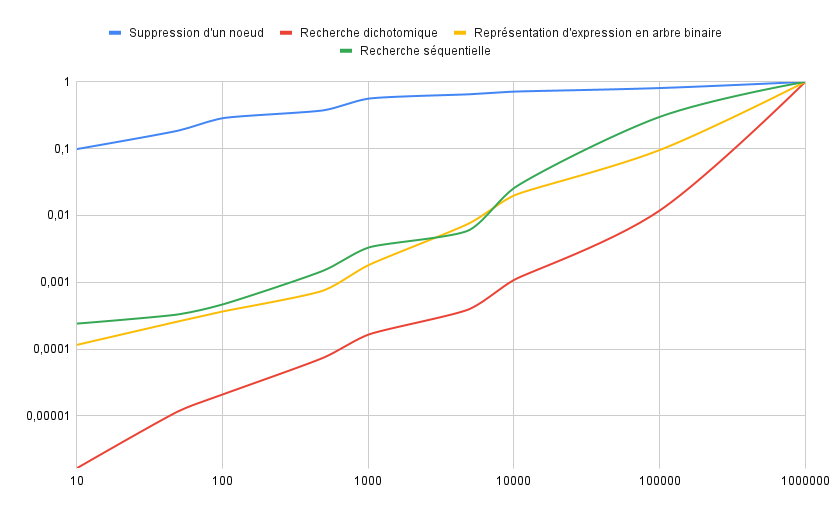
\includegraphics[scale=0.5]{./ressources/chartee.png}
        \caption{Comparaison des temps d'exécution des quatres algorithmes après mise à l'échelle}
    \label{fig:fig_conclusion}
\end{figure}
